
\section{时空的分类}
\subsection{外尔旋量的类光结构}

我们已经知道外尔旋量可以由一个对称旋量$\upPsi _{\boldsymbol{ABCD}}$表达,而根据定理(3.9),在流形的每一点$P$上,外尔旋量都有一个正则分解
\begin{equation*}
	\upPsi _{\boldsymbol{ABCD}} =\alpha _{(\boldsymbol{A}} \beta _{\boldsymbol{B}} \gamma _{\boldsymbol{C}} \delta _{\boldsymbol{D})} .
\end{equation*}
我们称类光方向$\alpha _{\boldsymbol{A}} ,\beta _{\boldsymbol{A}} ,\gamma _{\boldsymbol{A}} ,\delta _{\boldsymbol{A}}$为引力主类光方向(gravitational principal null directions, GPNDs)。除此之外,如果我们考虑$\xi ^{A} =( 1,z)$,那么
\begin{equation}
	\begin{aligned}
		\upPsi _{ABCD} \xi ^{A} \xi ^{B} \xi ^{C} \xi ^{D} & =\upPsi _{0} +4\upPsi _{1} z+6\upPsi _{2} z^{2} +4\upPsi _{3} z^{3} +\upPsi _{4} z^{4}\\
		& =(\alpha _{0} +z\alpha _{1} )(\beta _{0} +z\beta _{1} )(\gamma _{0} +z\gamma _{1} )(\delta _{0} +z\delta _{1} ),
	\end{aligned}
	\label{eq:5.93}
\end{equation}
即我们可以用\ref{eq:5.93}的根来确定GPNDs的重数,例如如果
\begin{equation*}
	\upPsi _{\boldsymbol{ABCD}} \xi ^{\boldsymbol{A}} \xi ^{\boldsymbol{B}} =0,
\end{equation*}
这代表最少有三个类光方向重合。如果我们给出$\xi ^{\boldsymbol{A}}$对应的矢量
\begin{equation*}
	v^{\boldsymbol{a}} =\pm \xi ^{\boldsymbol{A}}\overline{\xi }^{\boldsymbol{A} '} ,
\end{equation*}
那么就可以得到GPNDs的分类:

\begin{table}[h]
	\centering
	\begin{tabularx}{\textwidth}{KKK}
		\toprule 
		GPNDs的重数 & 旋量条件 & 张量条件 \\
		\midrule 
		单重 & $\upPsi _{\boldsymbol{ABCD}} \xi ^{\boldsymbol{A}} \xi ^{\boldsymbol{B}} \xi ^{\boldsymbol{C}} \xi ^{\boldsymbol{D}} =0$ & $v_{[\boldsymbol{f}} C_{\boldsymbol{a}]\boldsymbol{bc}[\boldsymbol{d}} v_{\boldsymbol{e}]} v^{\boldsymbol{b}} v^{\boldsymbol{c}} =0$ \\
		至少双重 & $\upPsi _{\boldsymbol{ABCD}} \xi ^{\boldsymbol{A}} \xi ^{\boldsymbol{B}} \xi ^{\boldsymbol{C}} =0$ & $C_{\boldsymbol{abc}[\boldsymbol{d}} v_{\boldsymbol{e}]} v^{\boldsymbol{b}} v^{\boldsymbol{c}} =0$ \\
		至少三重 & $\upPsi _{\boldsymbol{ABCD}} \xi ^{\boldsymbol{A}} \xi ^{\boldsymbol{B}} =0$ & $C_{\boldsymbol{abc}[\boldsymbol{d}} v_{\boldsymbol{e}]} v^{\boldsymbol{c}} =0$ \\
		四重 & $\upPsi _{\boldsymbol{ABCD}} \xi ^{\boldsymbol{A}} =0$ & $C_{\boldsymbol{abcd}} v^{\boldsymbol{c}} =0$ \\
		\bottomrule
		\end{tabularx}
	\caption{不同GPNDs对于外尔张量(旋量)的分类}
	\label{tab:classification of Weyl tensor}
\end{table}

当然,我们也可以直接用主类光旋量本身来分类旋量$\upPsi _{\boldsymbol{ABCD}}$:
\begin{equation}
	\begin{aligned}
		\text{I} =\{1111\} : & \upPsi _{\boldsymbol{ABCD}} =\alpha _{(\boldsymbol{A}} \beta _{\boldsymbol{B}} \gamma _{\boldsymbol{C}} \delta _{\boldsymbol{D})}\\
		\text{II} =\{211\} : & \upPsi _{\boldsymbol{ABCD}} =\alpha _{(\boldsymbol{A}} \alpha _{\boldsymbol{B}} \gamma _{\boldsymbol{C}} \delta _{\boldsymbol{D})}\\
		\text{D} =\{22\} : & \upPsi _{\boldsymbol{ABCD}} =\alpha _{(\boldsymbol{A}} \alpha _{\boldsymbol{B}} \beta _{\boldsymbol{C}} \beta _{\boldsymbol{D})}\\
		\text{III} =\{31\} : & \upPsi _{\boldsymbol{ABCD}} =\alpha _{(\boldsymbol{A}} \alpha _{\boldsymbol{B}} \alpha _{\boldsymbol{C}} \beta _{\boldsymbol{D})}\\
		\text{N} =\{4\} : & \upPsi _{\boldsymbol{ABCD}} =\alpha _{(\boldsymbol{A}} \alpha _{\boldsymbol{B}} \alpha _{\boldsymbol{C}} \alpha _{\boldsymbol{D})}\\
		\text{O} =\{-\} : & \upPsi _{\boldsymbol{ABCD}} =0.
	\end{aligned}
	\label{eq:5.94}
\end{equation}
这我们假设了$\alpha _{\boldsymbol{A}} ,\beta _{\boldsymbol{A}} ,\gamma _{\boldsymbol{A}} ,\delta _{\boldsymbol{A}}$都是不平行的非零旋量。我们称分类\ref{eq:5.94}为Petrov类型。如果用图形表示不同类型的曲率旋量之间的关系,我们有图\ref{fig:Petrov}。其中箭头指向的方向代表了更大的GPNDs的简并度。

\begin{figure}[h]
	\centering
	

\tikzset{every picture/.style={line width=0.75pt}} %set default line width to 0.75pt        

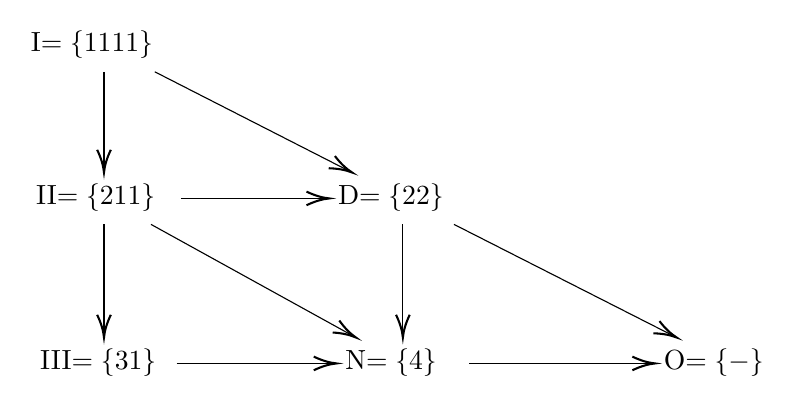
\begin{tikzpicture}[x=0.75pt,y=0.75pt,yscale=-1,xscale=1]
	%uncomment if require: \path (0,180); %set diagram left start at 0, and has height of 180
	
	
	
	% Text Node
	\draw (146,4) node [anchor=north west][inner sep=0.75pt]   [align=left] {I$=\{1111\}$};
	% Text Node
	\draw (148.5,77.5) node [anchor=north west][inner sep=0.75pt]   [align=left] {II$=\{211\}$};
	% Text Node
	\draw (294,77.5) node [anchor=north west][inner sep=0.75pt]   [align=left] {D$=\{22\}$};
	% Text Node
	\draw (150.5,157) node [anchor=north west][inner sep=0.75pt]   [align=left] {III$=\{31\}$};
	% Text Node
	\draw (297.5,157) node [anchor=north west][inner sep=0.75pt]   [align=left] {N$=\{4\}$};
	% Text Node
	\draw (451,157) node [anchor=north west][inner sep=0.75pt]   [align=left] {O$=\{-\}$};
	% Connection
	\draw    (182.5,25) -- (182.5,71.5) ;
	\draw [shift={(182.5,73.5)}, rotate = 270] [color={rgb, 255:red, 0; green, 0; blue, 0 }  ][line width=0.75]    (10.93,-3.29) .. controls (6.95,-1.4) and (3.31,-0.3) .. (0,0) .. controls (3.31,0.3) and (6.95,1.4) .. (10.93,3.29)   ;
	% Connection
	\draw    (206.99,25) -- (300.23,72.59) ;
	\draw [shift={(302.01,73.5)}, rotate = 207.04] [color={rgb, 255:red, 0; green, 0; blue, 0 }  ][line width=0.75]    (10.93,-3.29) .. controls (6.95,-1.4) and (3.31,-0.3) .. (0,0) .. controls (3.31,0.3) and (6.95,1.4) .. (10.93,3.29)   ;
	% Connection
	\draw    (219.5,86) -- (289,86) ;
	\draw [shift={(291,86)}, rotate = 180] [color={rgb, 255:red, 0; green, 0; blue, 0 }  ][line width=0.75]    (10.93,-3.29) .. controls (6.95,-1.4) and (3.31,-0.3) .. (0,0) .. controls (3.31,0.3) and (6.95,1.4) .. (10.93,3.29)   ;
	% Connection
	\draw    (182.5,98.5) -- (182.5,151) ;
	\draw [shift={(182.5,153)}, rotate = 270] [color={rgb, 255:red, 0; green, 0; blue, 0 }  ][line width=0.75]    (10.93,-3.29) .. controls (6.95,-1.4) and (3.31,-0.3) .. (0,0) .. controls (3.31,0.3) and (6.95,1.4) .. (10.93,3.29)   ;
	% Connection
	\draw    (217.5,165.5) -- (292.5,165.5) ;
	\draw [shift={(294.5,165.5)}, rotate = 180] [color={rgb, 255:red, 0; green, 0; blue, 0 }  ][line width=0.75]    (10.93,-3.29) .. controls (6.95,-1.4) and (3.31,-0.3) .. (0,0) .. controls (3.31,0.3) and (6.95,1.4) .. (10.93,3.29)   ;
	% Connection
	\draw    (205.14,98.5) -- (302.11,152.03) ;
	\draw [shift={(303.86,153)}, rotate = 208.9] [color={rgb, 255:red, 0; green, 0; blue, 0 }  ][line width=0.75]    (10.93,-3.29) .. controls (6.95,-1.4) and (3.31,-0.3) .. (0,0) .. controls (3.31,0.3) and (6.95,1.4) .. (10.93,3.29)   ;
	% Connection
	\draw    (326.5,98.5) -- (326.5,151) ;
	\draw [shift={(326.5,153)}, rotate = 270] [color={rgb, 255:red, 0; green, 0; blue, 0 }  ][line width=0.75]    (10.93,-3.29) .. controls (6.95,-1.4) and (3.31,-0.3) .. (0,0) .. controls (3.31,0.3) and (6.95,1.4) .. (10.93,3.29)   ;
	% Connection
	\draw    (351.11,98.5) -- (456.61,152.09) ;
	\draw [shift={(458.39,153)}, rotate = 206.93] [color={rgb, 255:red, 0; green, 0; blue, 0 }  ][line width=0.75]    (10.93,-3.29) .. controls (6.95,-1.4) and (3.31,-0.3) .. (0,0) .. controls (3.31,0.3) and (6.95,1.4) .. (10.93,3.29)   ;
	% Connection
	\draw    (358.5,165.5) -- (446,165.5) ;
	\draw [shift={(448,165.5)}, rotate = 180] [color={rgb, 255:red, 0; green, 0; blue, 0 }  ][line width=0.75]    (10.93,-3.29) .. controls (6.95,-1.4) and (3.31,-0.3) .. (0,0) .. controls (3.31,0.3) and (6.95,1.4) .. (10.93,3.29)   ;
	
\end{tikzpicture}
	\caption{根据主类光旋量方向的重合程度可以将外尔旋量分类成不同种类}
	\label{fig:Petrov}
\end{figure}

除此之外,根据外尔标量的定义,我们可以给出不同Petrov时空中,外尔标量为零的个数。如果我们选择$\xi ^{\boldsymbol{A}} =o^{\boldsymbol{A}}$,即$v^{\boldsymbol{a}} =l^{\boldsymbol{a}}$,那么
\begin{equation*}
	\upPsi _{\boldsymbol{ABCD}} o^{\boldsymbol{A}} o^{\boldsymbol{B}} o^{\boldsymbol{C}} o^{\boldsymbol{D}} =\upPsi _{0} ,
\end{equation*}
即如果时空为Petrov-I型,那么可以选择$\upPsi _{0} =0$。同样的,如果$l^{\boldsymbol{a}}$为Petrov-II型时空的主零方向,那么$\upPsi _{0} =\upPsi _{1} =0$。如果$l^{\boldsymbol{a}}$为Petrov-D型时空的第一个主零方向,且$n^{\boldsymbol{a}} =\iota ^{\boldsymbol{A}} \iota ^{\boldsymbol{A} '}$为第二个主零方向,那么除了$\upPsi _{0} =\upPsi _{1} =0$,我们还有$\upPsi _{4} =\upPsi _{3} =0$。同样的,III型和N型分别对应了$\upPsi _{0} =\upPsi _{1} =\upPsi _{2} =0$和$\upPsi _{0} =\upPsi _{1} =\upPsi _{2} =\upPsi _{3} =0$,而O型时空所有的外尔标量都为零,即共形平坦。


\subsection{哥德堡-萨赫定理}

现在我们考虑里奇张量为零,即黎曼张量与外尔张量重合的时空。这时我们有定理

\begin{them}[label={Goldberg-Sachs Theorem}]{哥德堡-萨赫定理(Goldberg-Sachs Theorem)}
	如果外尔张量是II型,且选择了$l^{\boldsymbol{a}}$作为主类光方向,即$\upPsi _{0} =\upPsi _{1} =0$,那么我们有
	\begin{equation*}
		\kappa =\sigma =0.
	\end{equation*}
	反之,如果$\kappa =\sigma =0$,那么
	\begin{equation*}
		\upPsi _{0} =\upPsi _{1} =0,
	\end{equation*}
	且外尔张量是II型。
\end{them}

\begin{proof}
	我们先来证明正命题。如果$\upPsi _{0} =\upPsi _{1} =0$,那么此时的比安基恒等式为
	\begin{equation*}
		\begin{cases}
			3\kappa \upPsi _{2} & =0\\
			D\upPsi _{2} & =-2\kappa \upPsi _{3} +3\rho \upPsi _{2}\\
			D\upPsi _{3} -\delta '\upPsi _{2} & =-\kappa \upPsi _{4} -2( \epsilon -\rho ) \upPsi _{3} +3\pi \upPsi _{2} ,
		\end{cases}
	\end{equation*}
	以及
	\begin{equation*}
		\begin{cases}
			3\sigma \upPsi _{2} & =0\\
			-\upDelta \upPsi _{2} & =2\sigma \upPsi _{3} -3\tau \upPsi _{2}\\
			D'\upPsi _{2} -\delta \upPsi _{3} & =-3\mu \upPsi _{2} -2( \tau -\beta ) \upPsi _{3} +\sigma \upPsi _{4} ,
		\end{cases}
	\end{equation*}
	由于时空不平坦,即$\upPsi _{2} ,\upPsi _{3} ,\upPsi _{4}$不全为零,那么$\kappa =\sigma =0$。
	
	
	
	现在来证明反论。由于标架有$6$个自由度,我们可以选择标架使得$\epsilon =0$,此时满足$\kappa =\sigma =0$,且包含这些量的里奇恒等式为
	\begin{equation}
		\begin{aligned}
			D\rho  & =\rho ^{2}\\
			\upPsi _{0} & =0\\
			D\tau  & =(\overline{\tau } +\pi )\rho +\upPsi _{1}
		\end{aligned}
	\end{equation}
	以及
	\begin{equation}
		\begin{aligned}
			D\beta  & =\overline{\rho } \beta +\upPsi _{1}\\
			\delta \rho  & =(\overline{\alpha } +\beta )\rho +(\rho -\overline{\rho } )\tau -\upPsi _{1} .
		\end{aligned}
	\end{equation}
	从\ref{eq:5.95}的第二个式子中我们给出$\upPsi _{0} =0$。此时,比安基恒等式为
	\begin{equation}
		\begin{aligned}
			D\upPsi _{1} & =4\rho \upPsi _{1}\\
			\delta \upPsi _{1} & =2(2\tau +\beta )\upPsi _{1} ,
		\end{aligned}
	\end{equation}
	以及$D,\delta $的对易子给出
	\begin{equation}
		D\delta -\delta D=(\overline{\pi } -\overline{\alpha } -\beta )D+\overline{\rho } \delta .
	\end{equation}
	现在,我们可以进一步选择规范使得$\tau =0$, 那么\ref{eq:5.97}给出
	\begin{equation*}
		\begin{cases}
			D\ln \upPsi _{1} & =4\rho ,\\
			\delta \ln \upPsi _{2} & =2\beta ,
		\end{cases}
	\end{equation*}
	故
	\begin{equation*}
		(D\delta -\delta D)\ln \upPsi _{1} =2D\beta -4\delta \rho .
	\end{equation*}
	现在,将上式的右侧带入\ref{eq:5.96}给出
	\begin{equation}
		(D\delta -\delta D)\ln \upPsi _{1} =2\overline{\rho } \beta -4(\overline{\alpha } +\beta )\rho +6\upPsi _{1} .
	\end{equation}
	然而,如果我们直接将对易子\ref{eq:5.98}应用在$\ln \upPsi _{1}$上,我们有
	\begin{equation}
		\begin{aligned}
			(D\delta -\delta D)\ln \upPsi _{1} & =(\overline{\pi } -\overline{\alpha } -\beta )D\ln \upPsi _{1} +\overline{\rho } \delta \ln \upPsi _{1}\\
			& =4(\overline{\pi } -\overline{\alpha } -\beta )\rho +2\beta \overline{\rho } .
		\end{aligned}
	\end{equation}
	为了保证\ref{eq:5.99}和\ref{eq:5.100}两侧相同,我们必须有
	\begin{equation*}
		\upPsi _{1} =\frac{2}{3}\overline{\pi } \rho ,
	\end{equation*}
	而\ref{eq:5.95}的第三式对于$\tau =0$有
	\begin{equation*}
		\upPsi _{1} =-\overline{\pi } \rho ,
	\end{equation*}
	这意味着我们必须有
	\begin{equation*}
		\upPsi _{1} =0.
	\end{equation*}
	至此正反两题证毕。
\end{proof}

哥德堡-萨赫定理的一个直接推论是,如果时空是Petrov-D型,那么当两个主类光方向$l^{\boldsymbol{a}} ,n^{\boldsymbol{a}}$重合时,即当且仅当
\begin{equation*}
	\upPsi _{0} =\upPsi _{1} =\upPsi _{3} =\upPsi _{4} =0
\end{equation*}
时,我们有
\begin{equation*}
	\kappa =\sigma =\nu =\lambda =0.
\end{equation*}
值得注意的是,广义相对论的黑洞解全部都是Petrov-D型的,因此我们总是能够令自旋系数$\kappa ,\sigma ,\lambda ,\nu $和除了$\upPsi _{2}$以外的外尔标量为零,这也是纽曼-彭罗斯形式对于它们特别有效的原因。